\section{Predictability Analysis}
\label{sec:dataAnalysis}

\begin{figure*}[!ht]
	\centering
%	\vspace{-0.3cm}
	\subfloat[PV generation]{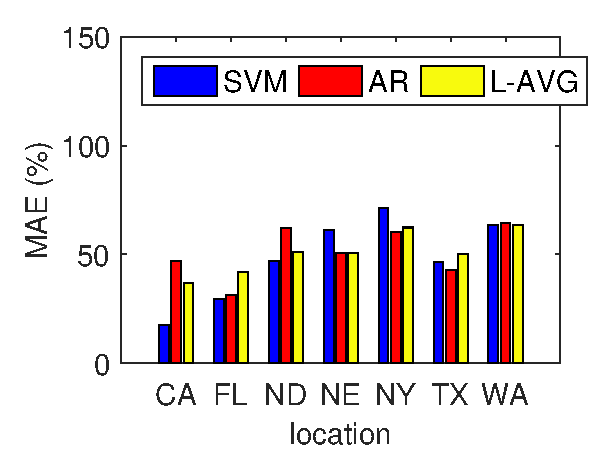
\includegraphics[width=.24\linewidth]{figs/svm_vs_ar_vs_avg_solar}}
	\subfloat[Wind generation]{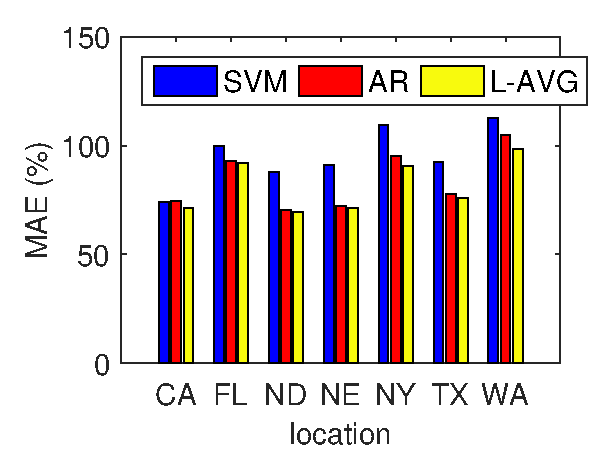
\includegraphics[width=.24\linewidth]{figs/svm_vs_ar_vs_avg_wind}}
	\subfloat[Electricity price]{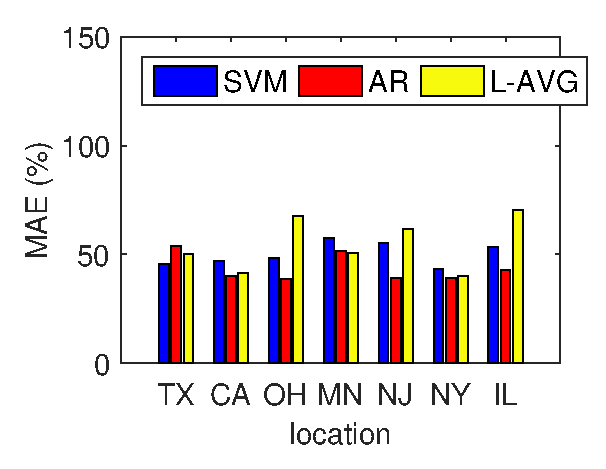
\includegraphics[width=.24\linewidth]{figs/svm_vs_ar_vs_avg_price}}
	\subfloat[Workload]{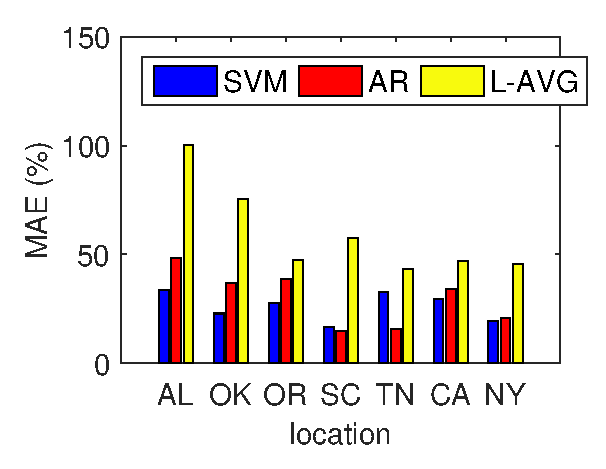
\includegraphics[width=.24\linewidth]{figs/svm_vs_ar_vs_avg_workload}}
	\caption{Comparisons of SVM, AR and L-AVG. The codes of US states are California (CA), Florida (FL), North Dakota (ND), Nebraska (NE), New York (NY), Texas (TX), Washington (WA), Ohio (OH), Minnesota (MN), New Jersey (NJ), Illinois (IL), Alabama (AL), Georgia (GA), Oklahoma (OK), South Carolina (SC), Virginia (VA), and Tennessee (TN).}
	\label{fig:CompareARandAVG}
%	\vspace{-0.5cm}
\end{figure*}

\diff{In this section, we study the long-term predictability of metrics
critical to our procurement systems for multi-timescale markets;
namely, workload, renewable generation, and real-time electricity
price. 
We design two long-term prediction methods, and analyse the prediction 
errors associated with each metric using real-world traces.
Our analysis also provides several insights into the nature of the
\emph{distributions} of these metrics.}

% The main purpose of our analysis is used as inputs for our proposed
% procurement systems and provide some insights into the long-term
% prediction errors associated with each metric.
For our study, we collected 3-year real-world traces of photovoltaic
(PV) generation, wind generation, and electricity prices for 20 states
of the US. The 3-year PV and wind generation data were downloaded
using the System Advisor Model (SAM) software, developed by the
National Renewable Energy Laboratory (NREL) \cite{nrel2010SAM}. The
3-year electricity price data are from different regional transmission
operators (RTOs) in the US, i.e., PJM, MISO, CAISO, ISONE, and NYSIO
\cite{qureshi2009cutting}. In addition, we collected 2-month workload
data for the same 20 states from Akamai Technologies, which serves
15-30\% of all Web content around the world from hundreds of data
centers around the world \cite{NygrenSS10}.

%In prior literature, prediction methods fall into one of the two categories: statistical methods and physical methods \cite{lei2009review}. The statistical methods or time-series-based methods exploit the correlation of data in the temporal domain to predict the future from the past data. The statistical methods include linear and non-linear regression models \cite{guoyang2005discussion}, Kalman filter \cite{louka2008improvements}, and machine learning techniques \cite{paoli2010forecasting, sfetsos2000univariate}. In the meantime, the physical methods use correlated physical conditions, such as geographical information, weather data, and time, to predict the future \cite{sharma2011predicting}. 

Long-term prediction is challenging for both statistical and physical
prediction methods \cite{lei2009review}. Statistical methods have to
deal with the weak correlation between the past and future
data. Meanwhile, physical methods require the input of physical
features that are often not available for long-term predictions. For
example, long-term weather forecast requires data from many parts of
the world which are only available in some specialized centers. %{\cite{wmoLongTermForecasting}}.
To improve the prediction accuracy,
prediction methods may exploit seasonality, such as annual
patterns. However, the effectiveness of using seasonality depends
heavily on the characteristics of the data.

%In order to design a prediction algorithm, it is necessary to understand the characteristics of the underlying data. Therefore, we first perform periodicity analysis over PV generation, wind generation, electricity prices, and workload respectively and the results are shown in Figure \ref{fig:periodgram}. The highest peaks occur at 24 hours in all the periodograms, which indicates the strong daily patterns of the data. %The behaviors of solar, wind, electricity price, and workload actually exhibit daily patterns. 

%As the long-term forecaster is a part of our energy procurement
%system, it is necessary to design a reliable long-term forecast method
%to produce the inputs for the energy procurement system. 
We design two long-term prediction methods to produce the inputs for
our energy procurement system: An autoregressive (AR) model and a
Support Vector Machine (SVM) model. The motivation for using the AR
method is to capture daily patterns and the correlation between past
and future data. On the other hand, we develop the SVM method to
capture the seasonality of the data.

In particular, our AR model predicts the value $x(day+d\_ah,hr)$ at
hour $hr$ for $d\_ah$ day-ahead based on the past $A$ days as
$x(day+d\_ah,hr) = \sum_{a=0}^{A-1} \omega_a x(day-a,hr) + c.$ The AR
model can obtain the coefficients $\omega_a$ and constant $c$ by
fitting the model to the historical data. We observe that it is not
necessary to pick a large value of $A$ for long-term prediction
because $A=7$ already achieves  competitive
performance. Additionally, $d\_ah$ is set at 30 days for PV
generation, wind generation, and electricity price, and at 1 day for
workload due to the limited length of data.


Our SVM model is designed to capture the seasonality of workload,
renewable generation, and electricity price.
% SVM is well-known as a learning algorithm for classification and
% regression analysis. JK -- not needed, in my opinion
%Similar to the work \cite{sharma2011predicting}, we focus the
%multi-class SVM that aims to estimate a predicted value based on given
%inputs. 
Similar to the work \cite{sharma2011predicting}, we use a multi-class
SVM. The first input to the SVM model is the average of the past $A$
days. The rest of inputs are the seasonality data, i.e., month of
year, day of month, day of week, and hour of day
\cite{deoras2010MatLabForecast}. For electricity generation from PV panels and wind turbines, we use month of year, day of month, and hour of day to
capture their seasonality. Similarly, we use month of year, day of
month, hour of day, and day of week in predicting electricity
prices. Due the limitation of the trace length, only day of week and
hour of day are used as the seasonality inputs for predicting
workload. The prediction window is the same as with the AR method,
i.e., 30 days for solar generation, wind generation, and electricity
prices, and 1 day for workload. The accuracy of SVM depends on the
selection of SVM kernel function and the kernel parameters. For each
set of data, we search for the best kernel function and the best
kernel parameters using LIBSVM, an SVM tool
\cite{chang2011libsvm}. The most suitable kernel function is Radial
Basis Function (RBF) but the kernel parameters differ for each
dataset.



\textbf{Prediction error analysis:} We now analyse the prediction errors under the AR and SVM methods.
%Prediction errors are used as a metric to quantify the performance of AR and SVM methods.
%Let $\hat{L}^r_j$, $\hat{w}^r_i$, and $\hat{p}^r_i$ denote long-term predicted values of renewable generation, workload, and electricity price. Further, let
%\begin{subequations}
%	\label{eq:predictionErrors}
%	\begin{align}
%		\varepsilon_i = {w}^r_i - \hat{w}^r_i, \\
%		\xi_j  = {L}^r_j - \hat{L}^r_j, \\
%		\epsilon_i = {p}^r_i - \hat{p}^r_i,
%	\end{align}
%\end{subequations}
%where $\varepsilon_i$, $\xi_j$, and $\epsilon_i$ are the prediction errors of renewable generation, workload, and electricity prices, respectively. 
We normalize the prediction errors by the average of real values and
show the values in percentage. For instance, a prediction error for PV
generation of 20 (-20) implies that we underestimate (overestimate)
the PV generation by 20\% of the average PV generation.

\desc{Comparison between SVM vs. AR vs. AVG}



We compare AR and SVM with a baseline method, long-term average
(L-AVG) {\cite{sinden2007characteristics}}. L-AVG assumes that the
long-term data has a long-term cycle. For example, PV generation may
have a yearly cycle. L-AVG takes the average of 30 days at the same
time over the past 2 years for PV generation, wind generation, and
electricity price. In particular, the predicted value at hour $hr$ of
day $day$ in $yr$ is computed as $x(yr, day,hr) =
\frac{1}{2}\sum_{y=1}^{2}\frac{1}{30}\sum_{d=15}^{-14}x(yr-y,day-d,hr)
.$ Assuming that user behavior has a weekly pattern, L-AVG takes the
averages of the workload demand at the same time of 7 days in the past
weeks. The mean absolute errors (MAEs) of three methods are
illustrated in Figure \ref{fig:CompareARandAVG}. In general, SVM and
AR do not perform better than L-AVG in predicting solar and wind
generation but they are better than L-AVG in predicting electricity
price, and workload. In predicting PV generation, SVM outperforms
others methods in some states like California that reveal the positive
impact of seasonality. However, some states like Washington (WA) and
New York (NY) having high precipitation can negatively affect the
performance of SVM and AR. Predicting wind generation is the hardest
among the four types of data as the prediction errors are very
large. It is because the wind generation often has very large
variation and fluctuation. On the other hand, SVM and AR are better
than L-AVG in terms of predicting electricity prices. AR is
surprisingly better than SVM in most states except for Texas (TX). The
seasonality in real-time electricity prices is not strong enough to
benefit SVM in long-term prediction. AR and SVM perform very well in
predicting workload compared to L-AVG in short-term. Overall, the
long-term prediction errors are relatively large compared to the mean
of measured data. Figure {\ref{fig:CompareARandAVG}} also highlights
that long prediction errors are dependent on locations, the types of
data, and the prediction methods. %

\begin{figure*}[pbth]
	\centering
%	\vspace{-0.3cm}
	\subfloat[PV generation]{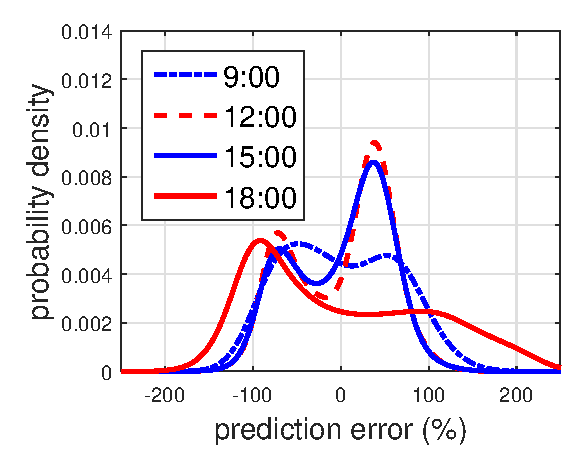
\includegraphics[width=.24\linewidth]{figs/ar_hourly_pdf_error_solar}}
	\subfloat[Wind generation]{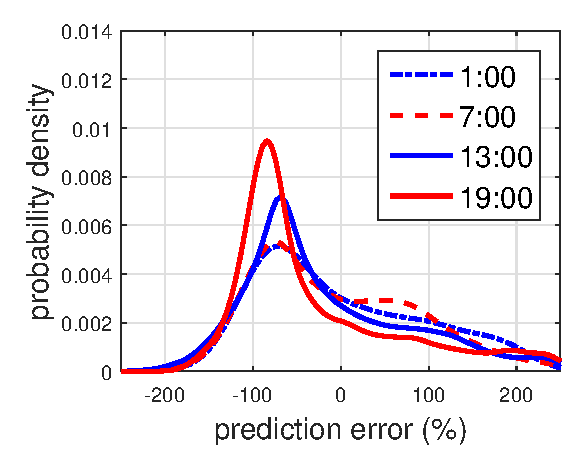
\includegraphics[width=.24\linewidth]{figs/ar_hourly_pdf_error_wind}}
	\subfloat[Electricity price]{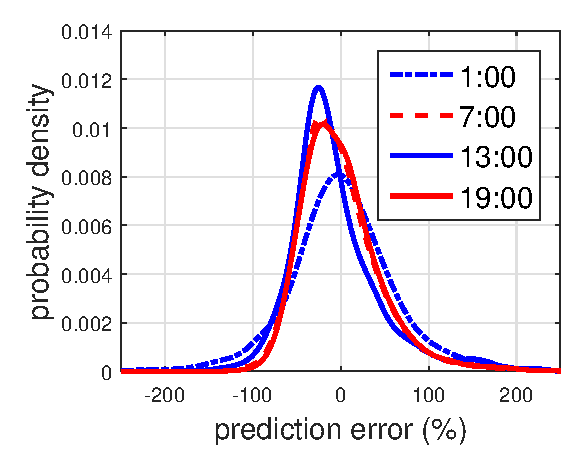
\includegraphics[width=.24\linewidth]{figs/ar_hourly_pdf_error_price}}
	\subfloat[Workload]{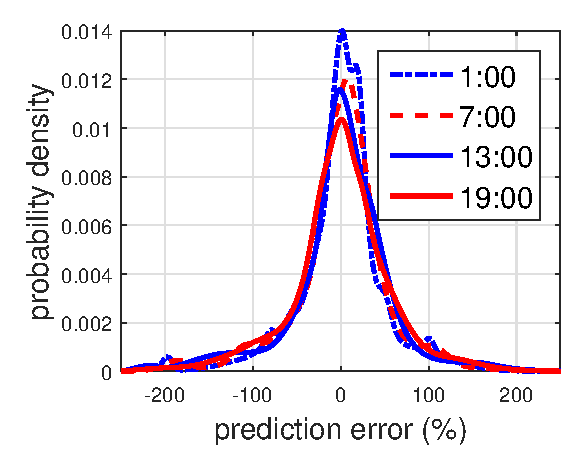
\includegraphics[width=.24\linewidth]{figs/ar_hourly_pdf_error_workload}}	
%	\vspace{-0.2cm}
	\caption{Probability density of prediction errors at different time of the day.}	
	\label{fig:hourlyDistribution}
%	\vspace{-0.4cm}
\end{figure*}

\textbf{What do the distributions of prediction errors look like?} Figure \ref{fig:hourlyDistribution} shows the probability density of the prediction errors at different times in a day of using the AR method. Each line represents the probability density of prediction errors during\delete{ an hour in a day}\new{ the same hour for all days}. The probability densities are obtained by averaging the probability densities of all the collected data. Our first observation is that prediction errors have zero-mean. However, the probability densities of PV generation, wind generation, electricity price, and workload are asymmetric. In particular, our prediction algorithms tend to over-predict wind generation with high probability as shown by the peaks around $-80$ in Figure \ref{fig:hourlyDistribution}(b). This is because wind generation is often low. Meanwhile, the peaks of electricity price prediction errors are close to zero-mean. The prediction errors of workload are more around zero. 

\begin{figure}[!ht]
	\centering
	%	\vspace{-0.4cm}
	\subfloat[PV generation]{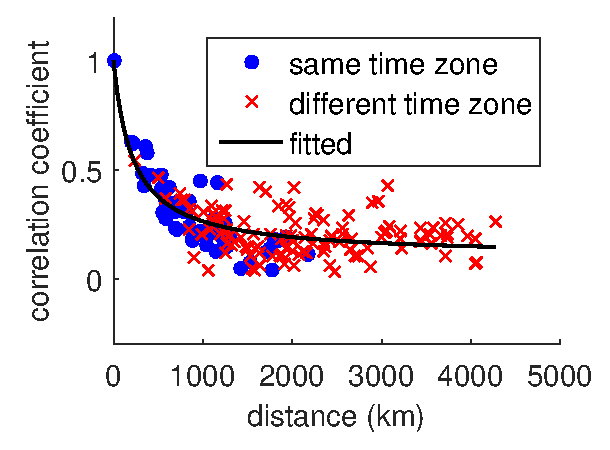
\includegraphics[width=.5\linewidth]{figs/solar_ar_corr_coff}}
	\subfloat[Wind generation]{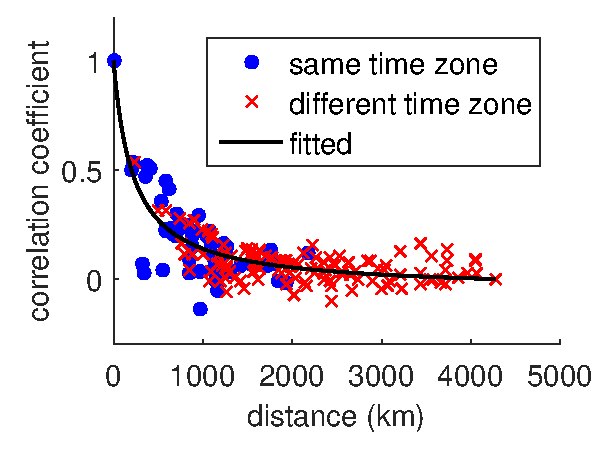
\includegraphics[width=.5\linewidth]{figs/wind_ar_corr_coff}}
	\\
	\subfloat[Electricity prices]{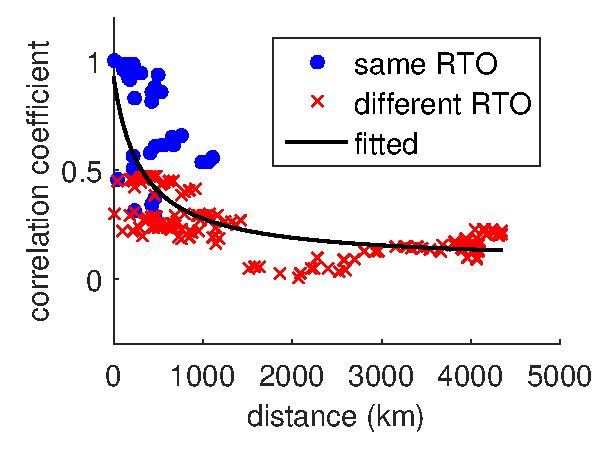
\includegraphics[width=.5\linewidth]{figs/price_ar_corr_coff}}
	\subfloat[Workload]{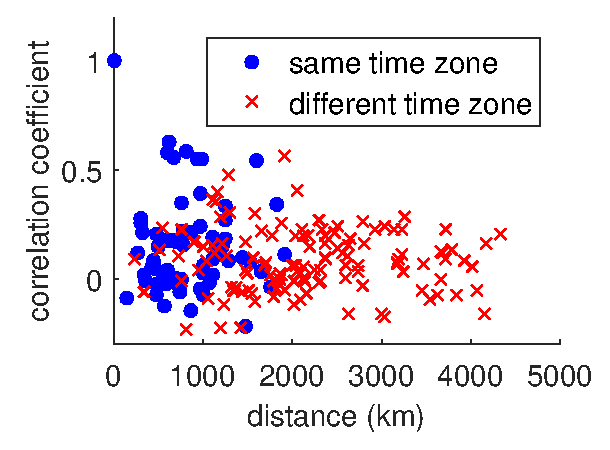
\includegraphics[width=.5\linewidth]{figs/workload_ar_corr_coff}}
	\caption{Correlation coefficients of prediction errors in spatial domain.}
	\label{fig:spaceCorrelation}
\end{figure}

\textbf{How correlated are the prediction errors in spatial domain?} The correlation of prediction errors in the spatial domain is of great interest to cloud providers with geo-distributed data centers. The correlation coefficients of prediction errors using AR with respect to the distance between two locations are shown in Figure \ref{fig:spaceCorrelation}. We classify PV generation, wind generation, and workload into two groups: within the same time zone or different time zones. There are also two groups of electricity prices: within the same RTO or different RTOs. Figure \ref{fig:spaceCorrelation} highlights that both distances \new{and groups can have the great impact on the correlation of prediction errors}\delete{the greater impact on the correlation than the groups have}. The prediction errors of PV and wind generation are strongly correlated (greater than 0.5) within 500 km, weakly correlated (less than 0.5) within 1000 km, and almost independent of each other when more than 1500 km apart. Note that electricity price is more correlated in the spatial domain than PV generation and wind generation due to the fact that some of the prices can be generated by the same RTO. However, the prediction errors of workload are uncorrelated with respect to distances and groups. This is because the workload depends on unpredictable user behavior and the dynamic Internet conditions.

